\documentclass{article}



\usepackage{fullpage}
\usepackage{nopageno}
\usepackage{amsmath}
\usepackage{amsfonts}
\usepackage{graphicx}
\usepackage{framed}
\usepackage{xcolor}

\definecolor{dark_red}{rgb}{0.5,0.0,0.0}
\definecolor{dark_green}{rgb}{0.0,0.5,0.0}
\definecolor{dark_blue}{rgb}{0.0,0.0,0.5}
\definecolor{blue}{rgb}{0.0,0.0,1.0}

\newcommand{\dr}[1]{\textcolor{dark_red}{#1}}
\newcommand{\dg}[1]{\textcolor{dark_green}{#1}}
\newcommand{\db}[1]{\textcolor{dark_blue}{#1}}
\newcommand{\blue}[1]{\textcolor{blue}{#1}}


\begin{document}

\section{Functions}

\begin{tabular}{cc}
\parbox{0.5\textwidth}{
A function is a mathematical object that accepts one or more quantities as ``input", and then returns a quantity as ``output". In the image to the right, a function \(f\) takes a single quantity \(x\) and returns the quantity \(f(x)\). The quantity \(x\) is often referred to as a ``parameter" of function \(f\). The set of input values \(x\) for which \(f(x)\) is defined is referred to as the {\bf domain} of \(f\). 
} & \parbox{0.5\textwidth}{

\includegraphics[width = 0.5\textwidth]{function_box}
}
\end{tabular}
Functions are generally defined by the notation:
\[\textbf{function\_name}(\textbf{parameter}) = \textbf{expression}\]
The ``\textbf{parameter}" is a symbol (often \(x\)) that is used as a placeholder for the input value in the expression that computes the output/return value. The ``\textbf{expression}" is an expression that involves the parameter symbol. The value of this expression when the parameter symbol is replaced with the input value is the output/return value.

\textbf{Examples:}
As an example function, let \(f\) be defined as \(f(X) = 2X+ 5\) for every \(X \in \mathbb{R}\). The domain of \(f\) is \(\mathbb{R}\). Some examples of using this function are:
\begin{itemize}
\item When the input is \(X = -4\), the return value is \(f(-4) = 2(-4) + 5 = -8 + 5 = -3\)
\item When the input is \(X = 0\), the return value is \(f(0) = 2(0) + 5 = 5\)
\item When the input is \(X = 15\), the return value is \(f(15) = 2(15) + 5 = 30 + 5 = 35\)
\item When the input is \(X = y + 2\), the return value is \(f(y + 2) = 2(y + 2) + 5 = (2y + 4) + 5 = 2y + 9\)
\end{itemize}

The choice of parameter symbol does not change the function. The definition \(f(y) = 2y + 5\) defines the same function as \(f(X) = 2X + 5\). It is more convenient to use a symbol that is not used for other purposes. We will often use capital letters \(X\), \(Y\), etc. to distinguish the parameter from other variables. The lowercase \(x\) for example, often sees other uses, and having a symbol other than \(x\) for the parameter name helps reduce ambiguity.

Use another function \(g\) defined by \(g(X) = \frac{8 - 3X}{7X + 2}\). The domain of \(g\) is all real numbers except for the value of \(X\) where \(7X + 2 = 0\).
\begin{itemize}
\item When the input is \(X = 2\), the return value is \(g(2) = \frac{8 - 3(2)}{7(2) + 2} = \frac{8 - 6}{14 + 2} = \frac{2}{16} = \frac{1}{8}\)
\item When the input is \(X = -1\), the return value is \(g(-1) = \frac{8 - 3(-1)}{7(-1) + 2} = \frac{8 + 3}{-7 + 2} = \frac{11}{-5} = -\frac{11}{5}\)
\item When the input is \(X = 0\), the return value is \(g(0) = \frac{8 - 3(0)}{7(0) + 2} = \frac{8}{2} = 4\) 
\item When the input is \(X = -2/7\), the return value is \(g(-2/7) = \frac{8 - 3(-2/7)}{7(-2/7) + 2} = \frac{56 + 6}{-14 + 14} = \frac{62}{0}\) which is undefined. \(-2/7\) is not part of the domain of \(g(X)\).
\end{itemize}



\subsection{Function Domains}

Given a function \(f\), the set of input values \(X\) for which \(f(X)\) is defined is referred to as the {\bf domain} of \(f\). 

Not every function has a domain that is the entire set of real numbers. For example, the function \(f(X) = \frac{1}{X}\) is not defined when \(X = 0\), so the domain is the set of all real numbers except \(0\): \(\mathbb{R} \setminus \{0\} = (-\infty, 0) \cup (0, +\infty)\). Also, (not considering complex numbers) the function \(f(X) = \sqrt{X}\) is not defined for negative values of \(X\) so the domain is the set of non-negative numbers: \([0, +\infty)\)


\subsection{Function Composition}

\begin{tabular}{cc}
\parbox{0.5\textwidth}{
Linking two functions together is referred to as ``function composition". The composition of two functions \(f\) followed by \(g\), denoted by \(g \circ f\) (this notation will not be used often), is a function that does the following: starting with the input parameter \(X\), function \(f\) is used to get \(f(X)\), and then function \(g\) is used to get \(g(f(X))\) which is the return value: \((g \circ f)(X) = g(f(X))\)  
} & \parbox{0.5\textwidth}{
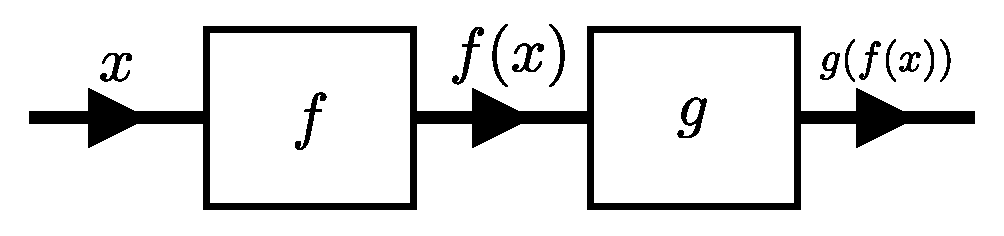
\includegraphics[width = 0.5\textwidth]{function_box_2_links} \\
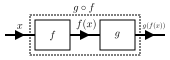
\includegraphics[width = 0.5\textwidth]{function_box_composition}
}
\end{tabular}
As in example of function composition, let function \(f\) be defined by \(f(X) = 6X - 7\), and function \(g\) be defined by \(g(X) = \frac{1}{2}X + \frac{1}{2}\). The composition of \(f\) followed by \(g\) is:
\[(g \circ f)(X) = g(f(X)) = g(6X - 7) = \frac{1}{2}(6X - 7) + \frac{1}{2} = 3X - 3\]

Below is shown the process of chaining together a large number of functions \(f_1, f_2, ..., f_N\) to get \(f_N \circ f_{N-1} \circ \dots \circ f_3 \circ f_2 \circ f_1\). Composing functions is how large expressions are created.

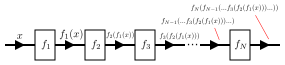
\includegraphics[width = \textwidth]{function_box_chain}

To assist with understanding what functions actually are, every arithmetic operator is a two-input function, and every expression is essentially a composition of simpler functions that are arithmetic operators.

In the image below, the expression \(\frac{5}{4 - 7x}\) is expressed by two different compositions of simple arithmetic steps. In the upper flow chart, \(x\) is first multiplied by \(-7\) via the function \(f_1(X) = -7X\) to get \(-7x\). \(-7x\) is then added to \(4\) via the function \(f_2(X) = 4 + X\) to get \(4 - 7x\). The reciprocal of \(4 - 7x\) is computed via the function \(f_3(X) = \frac{1}{X}\) to get \(\frac{1}{4 - 7x}\). Lastly, \(\frac{1}{4 - 7x}\) is multiplied by \(5\) via the function \(f_4(X) = 5X\) to get \(\frac{5}{4 - 7x}\). As an example, if \(x = 2\), then \(f_1(2) = -14\), \(f_2(-14) = -10\), \(f_3(-10) = -\frac{1}{10}\), and lastly \(f_4(-\frac{1}{10}) = -\frac{1}{2}\) so \(\frac{5}{4 - 7x} = -\frac{1}{2}\). 

In the lower flow chart, \(x\) is first multiplied by \(7\) via the function \(f_1(X) = 7X\) to get \(7x\). \(7x\) is then subtracted from \(4\) via the function \(f_2(X) = 4 - X\) to get \(4 - 7x\). Lastly, \(5\) is then divided by \(4 - 7x\) via the function \(f_3(X) = \frac{5}{X}\) to get \(\frac{5}{4 - 7x}\). As an example, if \(x = 2\), then \(f_1(2) = 14\), \(f_2(14) = -10\), and lastly \(f_3(-10) = -\frac{1}{2}\) so \(\frac{5}{4 - 7x} = -\frac{1}{2}\). 

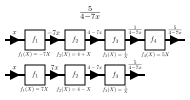
\includegraphics[width = \textwidth]{expressions_using_functions_1}

In the image below, \(x\) appears twice in the expression \(\frac{2x + 5}{6x - 7}\). The expressions \(2x + 5\) and \(6x - 7\) need to be separately computed before being divided via the two input function \(f_5(X, Y) = \frac{X}{Y}\). To compute \(2x + 5\) from \(x\), \(x\) is first multiplied by \(2\) via the function \(f_1(X) = 2X\) to get \(2x\). \(5\) is then added to \(2x\) via the function \(f_2(X) = X + 5\) to get \(2x + 5\). To compute \(6x - 7\) from \(x\), \(x\) is first multiplied by \(6\) via the function \(f_3(X) = 6X\) to get \(6x\). \(7\) is then subtracted from \(6x\) via the function \(f_4(X) = X - 7\) to get \(6x - 7\). With \(2x + 5\) and \(6x - 7\) computed, the two input function \(f_5(X, Y) = \frac{X}{Y}\) computes the quotient \(\frac{2x + 5}{6x - 7}\). As an example, if \(x = 1\), then \(f_1(1) = 2\), \(f_2(2) = 7\), \(f_3(1) = 6\), \(f_4(6) = -1\), and lastly \(f_5(7,-1) = -7\) so \(\frac{2x + 5}{6x - 7} = -7\)

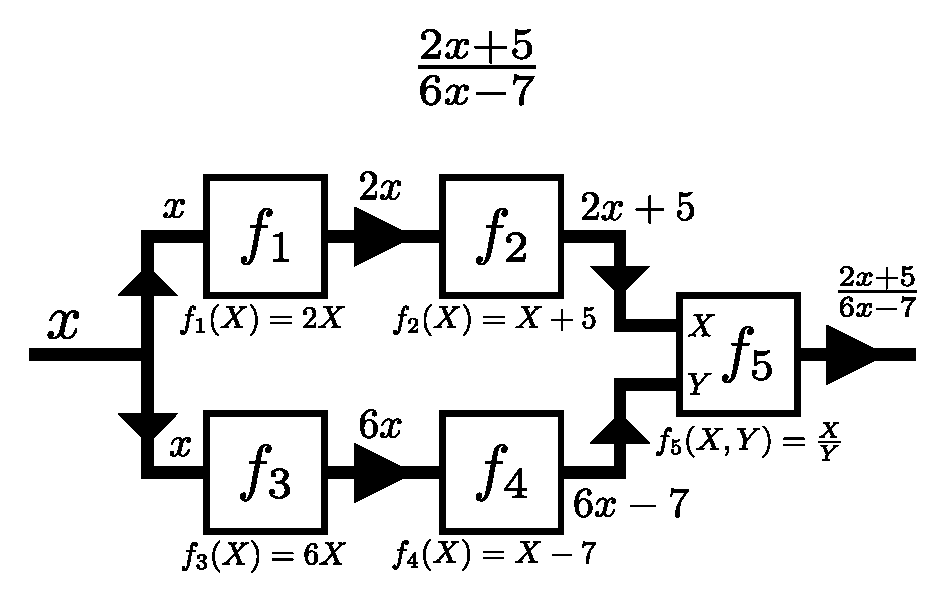
\includegraphics[width = 0.9\textwidth]{expressions_using_functions_2}




\section{Inverse Functions}

\begin{tabular}{cc}
\parbox{0.5\textwidth}{
The {\bf range} of a function \(f\) is the set of all possible output/return values:
\[\textbf{range} = \{f(x) | x \in \textbf{domain}\}\]
If a function is ``1 to 1", then no two different input values result in the same output value: 
\[\forall x,y \in \textbf{domain} : (x \neq y \implies f(x) \neq f(y))\]
For each value \(y\) from the range, there is exactly one input value \(x\) from the domain of \(f\) that generates \(y\). When a function \(f\) is ``1 to 1", the function \(f\) has an inverse. The inverse function of \(f\), denoted by \(f^{-1}\), ``reverses" function \(f\). The domain of \(f^{-1}\) is the range of \(f\), while the range of \(f^{-1}\) is the domain of \(f\). Given any value \(x\) from the range of \(f\), the value of \(f^{-1}(x)\) is the unique value from the domain of \(f\) such that \(f(f^{-1}(x)) = x\). For every value \(x\) from the domain of \(f\), applying \(f\) followed by \(f^{-1}\) brings \(x\) full circle: 
\[\forall x \in \textbf{domain} : f^{-1}(f(x)) = x\]
For every value \(x\) from the range of \(f\), applying \(f^{-1}\) followed by \(f\) also brings \(x\) full circle:
\[\forall x \in \textbf{range} : f(f^{-1}(x)) = x\] 
} & \parbox{0.5\textwidth}{
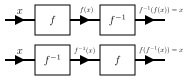
\includegraphics[width = 0.5\textwidth]{function_box_inverse} 
}
\end{tabular}

\textbf{Examples}
\begin{itemize}
\item Given for example the function \(f(X) = 3X\), the inverse function is \(f^{-1}(X) = \frac{X}{3}\). 
\item Given for example the function \(f(X) = X - 9\), the inverse function is \(f^{-1}(X) = X + 9\). 
\item The function \(f(X) = X^2\) is not 1 to 1, since \(f(x) = f(-x)\) for all values of \(x\). However, if the domain of \(f(X) = X^2\) is restricted to \([0, +\infty)\), then \(f\) has the inverse \(f^{-1}(X) = \sqrt{X}\), since the values of \(X\) that yield duplicate values have been excluded. If the domain were instead restricted to \((-\infty, 0]\), then \(f\) has the inverse \(f^{-1}(X) = -\sqrt{X}\).
\item The function \(f(X) = \sqrt{X}\) is 1 to 1, but the range is limited to \([0, +\infty)\). Therefore the domain of the inverse function \(f^{-1}(X) = X^2\) is restricted to \([0, +\infty)\).
\end{itemize}


\subsection{Inverting more complicated functions}

\begin{tabular}{cc}
\parbox{0.5\textwidth}{ 
Given the composition of two functions \(f\) followed by \(g\), denoted by \(g \circ f\) (for all \(X\), \((g \circ f)(X) = g(f(X))\)), to invert the combined function, the inverses are applied in the reverse order. If \(f\) is applied first, and then \(g\), to reverse the process, \(g\) is reversed first, followed by reversing \(f\):
\[(g \circ f)^{-1} = f^{-1} \circ g^{-1}\]
} & \parbox{0.5\textwidth}{
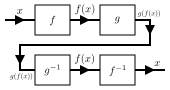
\includegraphics[width = 0.5\textwidth]{function_box_2_links_inverse} 
}
\end{tabular}

Consider a long chain of the functions \(f_1\), \(f_2\), \(f_3\), ..., \(f_N\) applied in the given order: \(f_N \circ ... \circ f_3 \circ f_2 \circ f_1\), the inverse is formed by applying the inverses of \(f_1\), \(f_2\), \(f_3\), ..., \(f_N\) in the reversed order:
\[(f_N \circ ... \circ f_3 \circ f_2 \circ f_1)^{-1} = f_1^{-1} \circ f_2^{-1} \circ f_3^{-1} \circ ... \circ f_N^{-1}\]

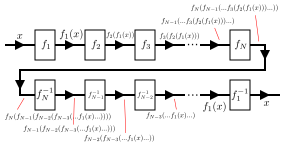
\includegraphics[width = \textwidth]{function_box_chain_inverse} 

\textbf{Examples}
\begin{itemize}
%%%%%%%%%%%%%%%%%%%%
\item The function \(g(X) = 3X - 7\) is the function \(f_1(X) = 3X\) followed by the function \(f_2(X) = X - 7\): \(g(X) = f_2(f_1(X))\). The inverses of \(f_1\) and \(f_2\) are respectively \(f_1^{-1}(X) = \frac{X}{3}\) and \(f_2^{-1}(X) = X + 7\). The inverse of \(g\) is: 
\[g^{-1}(X) = f_1^{-1}(f_2^{-1}(X)) = f_1^{-1}(X + 7) = \frac{X + 7}{3}\]
%%%%%%%%%%%%%%%%%%%%
\item The function \(g(X) = \frac{3}{-2X - 5}\) is the function \(f_1(X) = -2X\) followed by the function \(f_2(X) = X - 5\) followed by \(f_3(X) = \frac{1}{X}\) followed by \(f_4(X) = 3X\): \(g(X) = f_4(f_3(f_2(f_1(X))))\). The inverses of these functions are respectively \(f_1^{-1}(X) = \frac{X}{-2}\) and \(f_2^{-1}(X) = X + 5\) and \(f_3^{-1}(X) = \frac{1}{X}\) and \(f_4^{-1}(X) = \frac{X}{3}\). The inverse of \(g\) is: 
\begin{align*}
g^{-1}(X) = & f_1^{-1}(f_2^{-1}(f_3^{-1}(f_4^{-1}(X)))) 
= f_1^{-1}(f_2^{-1}(f_3^{-1}(\frac{X}{3})))  
= f_1^{-1}(f_2^{-1}(\frac{3}{X})) 
= f_1^{-1}(\frac{3}{X} + 5) 
= -\frac{3}{2X} - \frac{5}{2}
\end{align*} 
\end{itemize}



\section{Solving Equations}

Solving equations involves taking an equation with the form: 
\[\textbf{expression}_1 = \textbf{expression}_2\]
and manipulating the equation to have the form 
\[\textbf{variable} = \textbf{expression}\]
where the expression ``\textbf{expression}" computes the value of the variable ``\textbf{variable}". An equation is manipulated by deriving equations that are true if and only if the original equation is true. Given the equation \(A = B\) and any single input function \(f\) whose domain includes \(A\) and \(B\), then 
\[A = B \implies f(A) = f(B)\] 
The truth of \(A = B\) implies the truth of \(f(A) = f(B)\). However the reverse may not be true. It is not always the the case that the truth of \(f(A) = f(B)\) implies the truth of \(A = B\). A clear example uses the function \(f(x) = x^2\). The truth of \(x = 2\) implies that \(x^2 = 4\), but the truth of \(x^2 = 4\) does not imply that \(x = 2\), since \(x = -2\) is also a valid alternative. For the truth of \(f(A) = f(B)\) to imply \(A = B\), \(f\) must be 1 to 1 and have an inverse. When \(f\) is 1 to 1,
\[A = B \iff f(A) = f(B)\]
and the equation \(f(A) = f(B)\) can replace \(A = B\) with no loss of information.

Given a 1 to 1 function \(g\) and a value \(c\) from the range of \(g\), the equation \(g(x) = c\) is solved for \(x\) by simply applying the inverse of function \(g\) to both sides of the equation:
\[g(x) = c \iff g^{-1}(g(x)) = g^{-1}(c) \iff x = g^{-1}(x)\]
Now imagine that \(g\) is the composition of 1 to 1 single variable functions: \(g(x) = f_N(...f_3(f_2(f_1(x)))...)\). \(x\) can only appear once in the expression for \(g(x)\), or else functions with two or more inputs are needed to express \(g(x)\). The equation \(g(x) = c\) is equivalent to 
\[f_N(...f_3(f_2(f_1(x)))...) = c\] 
Variable \(x\) is ``unwrapped" by applying the inverse functions of \(f_1\), \(f_2\), \(f_3\), ..., \(f_N\) in the reverse order:
\begin{align*}
& f_N(f_{N-1}(f_{N-2}(...f_1(x)...))) = c \\
\iff & f_{N-1}(f_{N-2}(...f_1(x)...)) = f_N^{-1}(c) \\  
\iff & f_{N-2}(...f_1(x)...) = f_{N-1}^{-1}(f_N^{-1}(c)) \\
\cdots & \cdots\cdots\cdots\cdots\cdots\cdots\cdots\cdots\cdots\cdots \\
\iff & x = f_1^{-1}(...f_{N-2}^{-1}(f_{N-1}^{-1}(f_N^{-1}(c)))...)
\end{align*}

\textbf{Examples:}

Consider the equation:

\[\frac{5}{2(7 - \frac{4}{x})} = \frac{3}{10}\]

\begin{tabular}{cc}
\parbox{0.4\textwidth}{
In the image to the right, the expression \(\frac{5}{2(7 - \frac{4}{x})}\) is the composition of the functions \(f_1(X) = \frac{1}{X}\), followed by \(f_2(X) = -4X\), followed by \(f_3(X) = 7 + X\), followed by \(f_4(X) = 2X\), followed by \(f_5(X) = \frac{1}{X}\), lastly followed by \(f_6(X) = 5X\).
\[\frac{5}{2(7 - \frac{4}{x})} = f_6(f_5(f_4(f_3(f_2(f_1(x))))))\]
The inverses of the component functions are respectively \(f_1^{-1}(X) = \frac{1}{X}\); \(f_2^{-1}(X) = \frac{X}{-4}\); \(f_3^{-1}(X) = X - 7\); \(f_4^{-1}(X) = 2X\); \(f_5^{-1}(X) = \frac{1}{X}\); and \(f_6^{-1}(X) = 5X\). Applying the inverse functions in the reverse order to the equation \(\frac{5}{2(7 - \frac{4}{x})} = \frac{3}{10}\) yields:
\begin{align*}
& \frac{5}{2(7 - \frac{4}{x})} = \frac{3}{10} 
\iff \frac{1}{2(7 - \frac{4}{x})} = \frac{3}{50} \\
\iff & 2(7 - \frac{4}{x}) = \frac{50}{3} 
\iff 7 - \frac{4}{x} = \frac{25}{3} \\
\iff & -\frac{4}{x} = \frac{4}{3} 
\iff \frac{1}{x} = -\frac{1}{3} \\
\iff & x = -3
\end{align*}
} & \parbox{0.5\textwidth}{
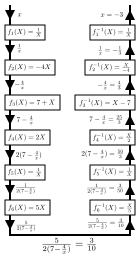
\includegraphics[width = 0.5\textwidth]{solving_equation_1}
}
\end{tabular}

The functions that comprise the expression that contains the variable to be solved for should be easily invertible. Easy functions to invert include:
\begin{itemize}
\item \(f(X) = X + a\) (simply add \(a\)) with the inverse \(f^{-1}(X) = X - a\) (simply subtract \(a\))
\item \(f(X) = a - X\) (simply subtract from \(a\)) with the inverse \(f^{-1}(X) = a - X\) (simply subtract from \(a\))
\item \(f(X) = aX\) where \(a \neq 0\) (simply multiply by \(a\)) with the inverse \(f^{-1}(X) = \frac{X}{a}\) (simply divide by \(a\))
\item \(f(X) = \frac{1}{X}\) (compute the reciprocal of \(X\)) with the inverse \(f^{-1}(X) = \frac{1}{X}\) (compute the reciprocal)
\item \(f(X) = \frac{a}{X}\) where \(a \neq 0\) (divide \(a\) by \(X\)) with the inverse \(f^{-1}(X) = \frac{a}{X}\) (divide \(a\) by \(X\))
\item \(f(X) = X^k\) where \(k\) is an odd natural number (raise to the \(k^\text{th}\) power) with the inverse \(f^{-1}(X) = \sqrt[k]{X}\) (compute the \(k^\text{th}\) root).
\end{itemize} 

When multiple instances of the desired variable are present, the equation must be manipulated until only one instance is present. Consider for example, the equation:
\[2a + 6 = 7a - 14\]
Subtracting \(2a\) from both sides gives \(6 = 5a - 14\), where \(a\) now only appears once. The expression that includes \(a\) can now be undone sequentially:
\begin{align*}
& 5a - 14 = 6
\iff 5a = 20 
\iff a = 4
\end{align*}

Consider the equation
\[\frac{4y - 3}{5 + 2y} = -2\]
The variable \(y\) appears twice, so to solve for \(y\), both sides must be multiplied by \(5 + 2y\) to eliminate the denominator:
\[\frac{4y - 3}{5 + 2y} = -2 \iff 4y - 3 = -2(5 + 2y) \iff 4y - 3 = -10 - 4y\]
Collecting \(y\) on the left side is done by adding \(4y\) to both sides and then adding the coefficients of \(y\):
\[4y - 3 = -10 - 4y \iff 8y - 3 = -10\]
Now \(y\) only appears once so the expression that includes \(y\) can now be undone sequentially:
\[8y - 3 = -10 \iff 8y = -7 \iff y = -\frac{7}{8}\]



\subsection{Solving equations with placeholder values}

Not every variable in an equation is to be solved for. Some values are left as symbols because:
\begin{itemize}
\item Their values have not yet been chosen. 
\item Or the values are left as symbols to avoid making approximations at this stage. 
\end{itemize}

Consider the equation
\[\frac{1}{(x(5-a) + 3b)^3 - x} = \frac{1}{2x}\]
Treating \(b\) and \(x\) as fixed quantities, the equation will first be solved for \(a\):

\begin{tabular}{cc}
\parbox{0.4\textwidth}{
\(a\) appears only once, and the functions that are used to generate the final expression that contains \(a\) are: \(f_1(X) = -X\), followed by \(f_2(X) = 5 + X\), followed by \(f_3(X) = xX\), followed by \(f_4(X) = X + 3b\), followed by \(f_5(X) = X^3\), followed by \(f_6(X) = X - x\), lastly followed by \(f_7(X) = \frac{1}{X}\). 
\begin{align*}
& \frac{1}{(x(5-a) + 3b)^3 - x} \\
= & f_7(f_6(f_5(f_4(f_3(f_2(f_1(a)))))))
\end{align*}
The inverses of the component functions are respectively \(f_1^{-1}(X) = -X\); \(f_2^{-1}(X) = X - 5\); \(f_3^{-1}(X) = \frac{X}{x}\); \(f_4^{-1}(X) = X - 3b\); \(f_5^{-1}(X) = \sqrt[3]{X}\); \(f_6^{-1}(X) = X + x\); and \(f_7^{-1}(X) = \frac{1}{X}\). Applying the inverse functions in the reverse order to the equation yields:
\begin{align*}
& \frac{1}{(x(5-a) + 3b)^3 - x} = \frac{1}{2x} \\
\iff & (x(5-a) + 3b)^3 - x = 2x \\
\iff & (x(5-a) + 3b)^3 = 3x \\
\iff & x(5-a) + 3b = \sqrt[3]{3x} \\
\iff & x(5-a) = -3b + \sqrt[3]{3x} \\
\iff & 5 - a = \frac{-3b + \sqrt[3]{3x}}{x} \\
\iff & -a = \frac{-3b + \sqrt[3]{3x}}{x} - 5 \\
\iff & a = \frac{3b - \sqrt[3]{3x}}{x} + 5
\end{align*}
} & \parbox{0.5\textwidth}{
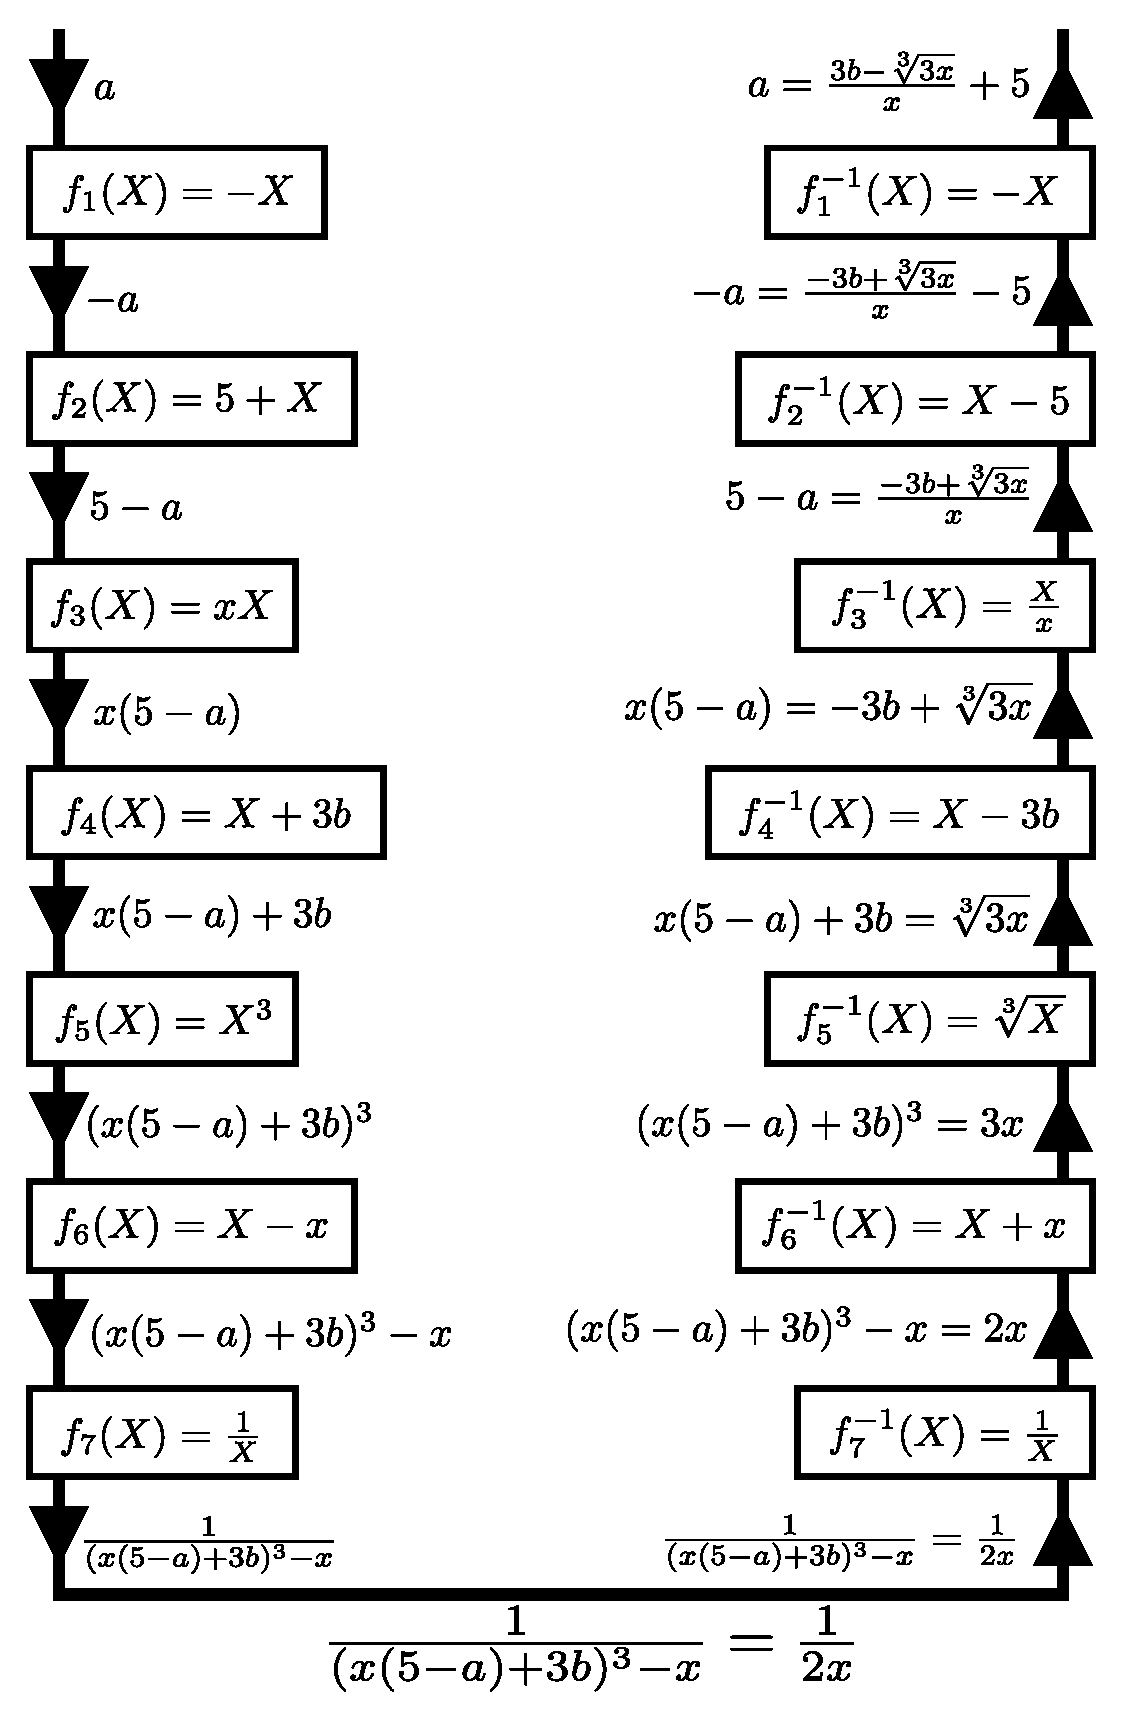
\includegraphics[width = 0.5\textwidth]{solving_equation_2}
}
\end{tabular}

Now treating \(a\) and \(x\) as fixed quantities, the equation will next be solved for \(b\):

\begin{tabular}{cc}
\parbox{0.4\textwidth}{
\(b\) appears only once, and the functions that are used to generate the final expression that contains \(b\) are: \(f_1(X) = 3X\), followed by \(f_2(X) = x(5 - a) + X\), followed by \(f_3(X) = X^3\), followed by \(f_4(X) = X - x\), lastly followed by \(f_5(X) = \frac{1}{X}\). 
\begin{align*}
& \frac{1}{(x(5-a) + 3b)^3 - x} \\
= & f_5(f_4(f_3(f_2(f_1(b)))))
\end{align*}
The inverses of the component functions are respectively \(f_1^{-1}(X) = \frac{X}{3}\); \(f_2^{-1}(X) = X - x(5 - a)\); \(f_3^{-1}(X) = \sqrt[3]{X}\); \(f_4^{-1}(X) = X + x\); and \(f_5^{-1}(X) = \frac{1}{X}\). Applying the inverse functions in the reverse order to the equation yields:
\begin{align*}
& \frac{1}{(x(5-a) + 3b)^3 - x} = \frac{1}{2x} \\
\iff & (x(5-a) + 3b)^3 - x = 2x \\
\iff & (x(5-a) + 3b)^3 = 3x \\
\iff & x(5-a) + 3b = \sqrt[3]{3x} \\
\iff & 3b = x(a-5) + \sqrt[3]{3x} \\
\iff & b = \frac{x(a-5) + \sqrt[3]{3x}}{3}
\end{align*}
} & \parbox{0.5\textwidth}{
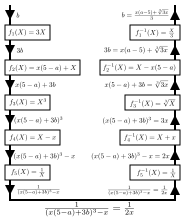
\includegraphics[width = 0.5\textwidth]{solving_equation_3}
}
\end{tabular}

\textbf{Another example:}

Consider the equation 

\[3ac + 5a - 4c = 2c\]

Solving for \(a\), while treating \(c\) as a placeholder symbol gives:

\begin{align*}
& 3ac + 5a - 4c = 2c \\
\iff & (3c + 5)a - 4c = 2c 
\iff (3c + 5)a = 6c 
\iff a = \frac{6c}{3c + 5}
\end{align*}

Solving for \(c\), while treating \(a\) as a placeholder symbol gives:

\begin{align*}
& 3ac + 5a - 4c = 2c 
\iff 3ac + 5a - 6c = 0 \\
\iff & (3a - 6)c + 5a = 0 
\iff (3a - 6)c = -5a 
\iff c = \frac{-5a}{3a - 6}
\end{align*}



\textbf{Another example:}

Consider the equation

\[4a^3 + \frac{1}{x} = 7 - 2a^3 - \frac{3}{x}\]

Solving for \(a\), while treating \(x\) as a placeholder symbol gives:

\begin{align*}
& 4a^3 + \frac{1}{x} = 7 - 2a^3 - \frac{3}{x} \\
\iff & 6a^3 + \frac{1}{x} = 7 - \frac{3}{x} 
\iff 6a^3 = 7 - \frac{4}{x} 
\iff a^3 = \frac{7}{6} - \frac{2}{3x} 
\iff a = \sqrt[3]{\frac{7}{6} - \frac{2}{3x}}
\end{align*}

Solving for \(x\), while treating \(a\) as a placeholder symbol gives:

\begin{align*}
& 4a^3 + \frac{1}{x} = 7 - 2a^3 - \frac{3}{x} \\
\iff & 4a^3 + \frac{4}{x} = 7 - 2a^3 
\iff \frac{4}{x} = 7 - 6a^3 
\iff \frac{1}{x} = \frac{7 - 6a^3}{4} 
\iff x = \frac{4}{7 - 6a^3}
\end{align*}



\textbf{Another example:}

Consider the equation

\[\frac{-9x + 5y - 7}{b + 2} = x(b + 2)^2\]

Solving for \(b\), while treating \(x\) and \(y\) as placeholder symbols gives:

\begin{align*}
& \frac{-9x + 5y - 7}{b + 2} = x(b + 2)^2 \\
\iff & x(b + 2)^3 = -9x + 5y - 7 
\iff (b + 2)^3 = \frac{-9x + 5y - 7}{x} 
\iff b + 2 = \sqrt[3]{\frac{-9x + 5y - 7}{x}} \\
\iff & b = -2 + \sqrt[3]{\frac{-9x + 5y - 7}{x}} 
\end{align*}

Solving for \(x\), while treating \(b\) and \(y\) as placeholder symbols gives:

\begin{align*}
& \frac{-9x + 5y - 7}{b + 2} = x(b + 2)^2 
\iff \frac{5y - 7}{b + 2} = \frac{9x}{b + 2} + x(b + 2)^2 \\ 
\iff & \left(\frac{9}{b + 2} + (b + 2)^2\right)x = \frac{5y - 7}{b + 2} 
\iff x = \frac{5y - 7}{(b + 2)\left(\frac{9}{b + 2} + (b + 2)^2\right)} 
\iff x = \frac{5y - 7}{9 + (b + 2)^3} 
\end{align*}

Solving for \(y\), while treating \(b\) and \(x\) as placeholder symbols gives:
\begin{align*}
& \frac{-9x + 5y - 7}{b + 2} = x(b + 2)^2 
\iff -9x + 5y - 7 = x(b + 2)^3 
\iff 5y = 9x + 7 + x(b + 2)^3 \\
\iff & y = \frac{9x + 7 + x(b + 2)^3}{5}
\end{align*}


\subsection{Traveling Example}

Consider the following scenario. With two available speeds, a slow speed \(v_\text{slow}\) and a fast speed \(v_\text{fast}\), the aim is to traverse a total distance \(D\) in \emph{exactly} total time \(T\). As of now, the quantities \(v_\text{slow}\), \(v_\text{fast}\), \(D\), and \(T\) have not yet been chosen, and are expressed using their respective symbols for now. The first leg of the journey will involve traveling at the slow speed \(v_\text{slow}\) for an unknown time \(t\), followed by traveling at the fast speed for the remaining time \(T - t\). The desired quantity to be solved for is the time \(t\) for which the slow speed is used. To find \(t\), the value of \(t\) will be used to derive various quantities until a limitation is apparent which will constitute the equation that will be solved for \(t\). The distance traveled in the first leg is \(v_\text{slow} t\), while the distance traveled in the remaining time \(T - t\) is \(v_\text{fast}(T - t)\). The total traveled distance is required to be \(D\), which yields the equation: 
\[v_\text{slow} t + v_\text{fast}(T - t) = D\]
Solving this equation for \(t\) yields:
\begin{align*}
& v_\text{slow} t + v_\text{fast}(T - t) = D 
\iff v_\text{slow} t + v_\text{fast}T - v_\text{fast} t = D \\
\iff & (v_\text{slow} - v_\text{fast})t + v_\text{fast}T = D 
\iff (v_\text{slow} - v_\text{fast})t = D - v_\text{fast}T 
\iff t = \frac{D - v_\text{fast}T}{v_\text{slow} - v_\text{fast}}
\end{align*}

Therefore:
\[t = \frac{D - v_\text{fast}T}{v_\text{slow} - v_\text{fast}}\]
is the time that should be spent traveling at the slower speed. 

Now for some numbers. Let \(v_\text{slow} = 1.561\text{m/s}\), \(v_\text{fast} = 5.342\text{m/s}\), \(D = 4000\text{m}\), and \(T = 2000\text{s}\). Substituting these quantities into the computed expression for \(t\) gives:
\[t = \frac{D - v_\text{fast}T}{v_\text{slow} - v_\text{fast}} = \frac{4000\text{m} - (5.342\text{m/s})(2000\text{s})}{1.561\text{m/s} - 5.342\text{m/s}} \approx \frac{-6684\text{m}}{-3.781\text{m/s}} \approx 1768\text{s}\]


\subsection{Mixing Example}

\begin{tabular}{cc}
\parbox{0.5\textwidth}{
Given a volume \(V_0\) of salt water with a salt concentration of \(c_0\), and another volume \(V_1\) of salt water with concentration \(c_1\), mixing the two volumes gives a mixture with volume \(V_0 + V_1\) and concentration of \(c_2\). The total mass of salt before mixing is \(c_0 \cdot V_0 + c_1 \cdot V_1\), and the total mass of salt after mixing is \(c_2(V_0 + V_1)\). Since the mass does not change during mixing, the following equation holds:
\[c_0 \cdot V_0 + c_1 \cdot V_1 = c_2(V_0 + V_1)\]
} & \parbox{0.5\textwidth}{
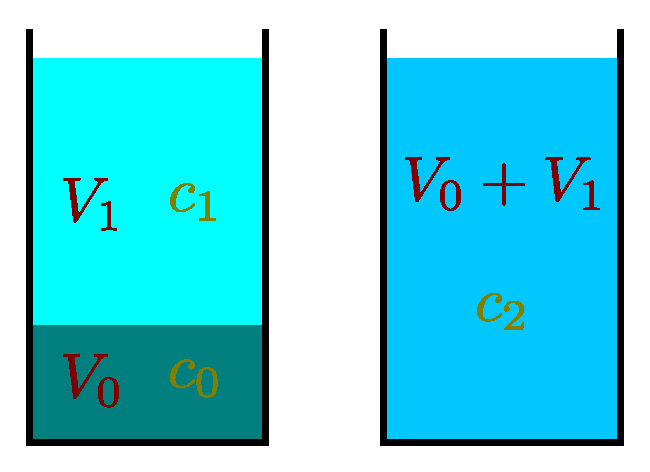
\includegraphics[width = 0.5\textwidth]{mixing_example}
}
\end{tabular}

If we know the volumes \(V_0\) and \(V_1\), and the concentrations \(c_0\) and \(c_1\), and are interested in the final concentration \(c_2\), the above equation can be solved for \(c_2\) which yields: 
\[c_0 \cdot V_0 + c_1 \cdot V_1 = c_2(V_0 + V_1) \iff c_2 = \frac{c_0 \cdot V_0 + c_1 \cdot V_1}{V_0 + V_1}\]

If we know volume \(V_0\) and concentrations \(c_0\) and \(c_1\), but are instead interested in finding the volume \(V_1\) needed to achieve a target final concentration of \(c_2\), the equation can instead be solved for \(V_1\) which yields:
\begin{align*}
& c_0 \cdot V_0 + c_1 \cdot V_1 = c_2(V_0 + V_1) \\
\iff & c_0 \cdot V_0 + c_1 \cdot V_1 = c_2 \cdot V_0 + c_2 \cdot V_1 \\
\iff & c_0 \cdot V_0 - c_2 \cdot V_0 = c_2 \cdot V_1 - c_1 \cdot V_1 \\
\iff & (c_2 - c_1)V_1 = (c_0 - c_2)V_0 \\
\iff & V_1 = \frac{c_0 - c_2}{c_2 - c_1}V_0
\end{align*}

\vspace{5mm}

If \(V_0 = 3.5\text{L}\); \(V_1 = 2.5\text{L}\); \(c_0 = 0.1\text{g/mL}\); \(c_1 = 0.01\text{g/mL}\); then to compute \(c_2\) we must first standardize the units: Replace \(\text{g/mL}\) with \(\frac{\text{g}}{10^{-3}L} = 10^3\text{g/L}\), or replace \(\text{L}\) with \(10^3\text{mL}\). It is simpler to replace \(\text{L}\) with \(10^3\text{mL}\), so volume is measured in \(\text{mL}\)'s, and concentration is measured in \(\text{g/mL}\). Hence

\[V_0 = 3.500 \times 10^3\text{mL} \;;\; V_1 = 2.500 \times 10^3\text{mL} \;;\; c_0 = 1.000 \times 10^{-1}\text{g/mL} \;;\; c_1 = 1.000 \times 10^{-2}\text{g/mL}\]

\begin{align*}
c_2 = & \frac{c_0 \cdot V_0 + c_1 \cdot V_1}{V_0 + V_1} 
= \frac{(3.500 \times 10^2\text{g}) + (2.500 \times 10^1\text{g})}{6.000 \times 10^3\text{mL}} 
= \frac{3.750 \times 10^2\text{g}}{6.000 \times 10^3\text{mL}} 
\approx 6.250 \times 10^{-2}\text{g/mL} \\
= & 0.06250 \text{g/mL}
\end{align*}

\vspace{5mm}

If \(V_0 = 3.5\text{L}\); \(c_0 = 0.1\text{g/mL}\); \(c_1 = 0.01\text{g/mL}\); and \(c_2 = 0.05\text{g/mL}\); then to compute \(V_1\) we must first standardize the units: replace \(\text{L}\) with \(10^3\text{mL}\), so volume is measured in \(\text{mL}\)'s, and concentration is measured in \(\text{g/mL}\). Hence 

\[V_0 = 3.500 \times 10^3\text{mL} \;;\; c_0 = 1.000 \times 10^{-1}\text{g/mL} \;;\; c_1 = 1.000 \times 10^{-2}\text{g/mL} \;;\; c_2 = 5.000 \times 10^{-2}\text{g/mL}\]

\begin{align*}
V_1 = & \frac{c_0 - c_2}{c_2 - c_1}V_0
= \frac{5.000 \times 10^{-2}\text{g/mL}}{4.000 \times 10^{-2}\text{g/mL}} (3.500 \times 10^3\text{mL})
= (1.250)(3.500 \times 10^3\text{mL}) 
\approx 4.375 \times 10^3\text{mL} \\
= & 4.375 \text{L}
\end{align*}


\end{document}













